\documentclass[11pt]{article}

\usepackage[margin=1in]{geometry}
\usepackage{amsmath}
\usepackage{amssymb}
\usepackage{mathpazo}
\usepackage{booktabs}
\usepackage{xcolor}
\usepackage{pgfplots}
\pgfplotsset{compat=1.17, every axis/.append style={font=\small}}
\usepackage{hyperref}

\emergencystretch=1.5em

\definecolor{kblue}{RGB}{42,120,214}
\definecolor{korange}{RGB}{235,104,52}
\definecolor{kteal}{RGB}{27,175,122}
\definecolor{kred}{RGB}{227,73,72}
\definecolor{kgray}{RGB}{136,135,128}

\title{Mathematical Foundations: A Teaching Companion \\
\large Six plain-language lessons with worked toy examples \\
Emission-Trajectory ML Project}
\author{Dr. Khawar Naeem \\ Qatar Transportation and Traffic Safety Center (QTTSC), Qatar University}
\date{29 August 2026}

\begin{document}
\maketitle

\begin{abstract}
This document re-teaches the mathematics of the project's foundations
document, \texttt{main.pdf} in the \texttt{math} folder (31 numbered
equations), as six plain-language lessons, each built around a small worked example that can
be computed by hand and re-used in front of an audience. It is a companion
for teaching and study, not a replacement for the formal document: every
lesson cites the equation numbers of \texttt{main.pdf}, and the formal
statements there remain authoritative. The lessons follow the order of the
foundations document: evaluation metrics, baselines, ordinary least
squares and Ridge, trees and boosting through XGBoost, uncertainty of a
skill score, and error decomposition. Each lesson ends with teach-back
questions; brief model answers are collected in the appendix. Prepared
with Claude (Anthropic) from live tutoring sessions in August 2026.
\end{abstract}

\tableofcontents

\section{How to use this document}

Each lesson has the same shape: the concept in plain words, the equations
with every symbol explained, one small worked example with numbers you can
verify by hand, a figure showing the mechanism, the trap that catches
students, and teach-back questions. The toy numbers are invented for
clarity and are labeled as such; every claim about the real project is
tied to the frozen results in \texttt{results/model\_comparison.csv} and
the Session 6 tables. Read with \texttt{main.pdf} open beside this
document; equation numbers cited here refer to it.

\section{Lesson 1: The referee. Five metrics are five different judges}

\subsection{Concept}

A single miss is easy to describe: the forecast said 970, reality was
1000, the miss is 30. The mathematics becomes interesting only when
hundreds of misses must be summarized in one number, because then someone
must decide whose misses count more. Every metric in the foundations
document (Equations 1 to 5) is a different answer to that one question,
and none of the answers is neutral.

\subsection{The pocket example}

Five countries, one year, one prediction each from the model and from
persistence (the rule ``next year equals this year''). Persistence's
prediction is last year's value, so its miss is the actual year-over-year
change. The numbers are invented for teaching.

\begin{center}
\begin{tabular}{lrrrrr}
\toprule
Country & Last year & Actual & Model predicts & Model miss & Persistence miss \\
\midrule
A (very large) & 965  & 1000 & 970  & 30 & 35 \\
B (large)      & 105  & 100  & 104  & 4  & 5 \\
C (mid)        & 53   & 50   & 48   & 2  & 3 \\
D (small)      & 12.5 & 10   & 11   & 1  & 2.5 \\
E (near zero)  & 2.5  & 0.5  & 1.5  & 1  & 2 \\
\bottomrule
\end{tabular}
\end{center}

\subsection{The five judges}

\textbf{MAE (Equation 1), the average miss.}
$\mathrm{MAE} = (30+4+2+1+1)/5 = 7.6$. Of the 38 total error units, 30
come from country A alone, which is 79 percent of the verdict decided by
one country. MAE is a democracy in which votes are weighted by tonnage.
This is a choice, not a flaw, and it is why the project's real MAE numbers
are dominated by the largest emitters.

\textbf{RMSE (Equation 2), the disaster detector.}
$\mathrm{RMSE} = \sqrt{(900+16+4+1+1)/5} = \sqrt{184.4} \approx 13.6$.
Squaring before averaging makes a miss of 30 contribute 900, so large
misses count quadratically extra. The useful diagnostic is the ratio to
MAE: if all five misses were identical, RMSE would equal MAE; here the
ratio is about 1.8, which signals that the error budget sits in a fat
tail of a few large misses. In the real project, \texttt{hgb\_level}
showed validation MAE 18.9 against RMSE 142.7, and that ratio alone
indicated catastrophic misses on giants before any per-country table was
opened.

\textbf{MedianAE (Equation 3), the typical country's experience.}
Sort the misses (1, 1, 2, 4, 30) and take the middle one: 2. Country A's
miss could grow from 30 to 3000 and this number would not move. The same
model is ``off by 7.6 on average'' and ``off by 2 for the typical
country,'' and both statements are true; the gap between them measures
how concentrated the errors are \cite{hyndman2006another}.

\textbf{MdAPE (Equation 4), the miss relative to the country's own size.}
Divide each miss by the country's own level: A scores $30/1000 = 3$
percent, B 4 percent, C 4 percent, D 10 percent, and E explodes to
$1/0.5 = 200$ percent because the denominator is nearly zero. Two
teachable events occur at once. First, the ranking reverses: A has the
largest absolute miss and the smallest percentage miss. Second, E shows
why the threshold $\tau = 1$ Mt is part of the metric's definition rather
than optional cleaning: with E excluded, MdAPE is the median of (3, 4, 4,
10), which is 4 percent. In the real test set, the same reversal appears
with Russia (a top-10 absolute miss at the sample's lowest percentage
error) against Pakistan and Vietnam.

\textbf{Skill (Equation 5), error relative to doing nothing.}
Persistence's misses sum to 47.5, so its MAE is 9.5, and
\[
\mathrm{Skill} = 1 - \frac{7.6}{9.5} = +0.2 .
\]
The reading: the model removed 20 percent of the error that ``assume no
change'' would have made. Zero means the model added nothing; one is the
unreachable perfect forecast; negative skill is a loss and must be
reported as one.

\begin{figure}[ht]
\centering
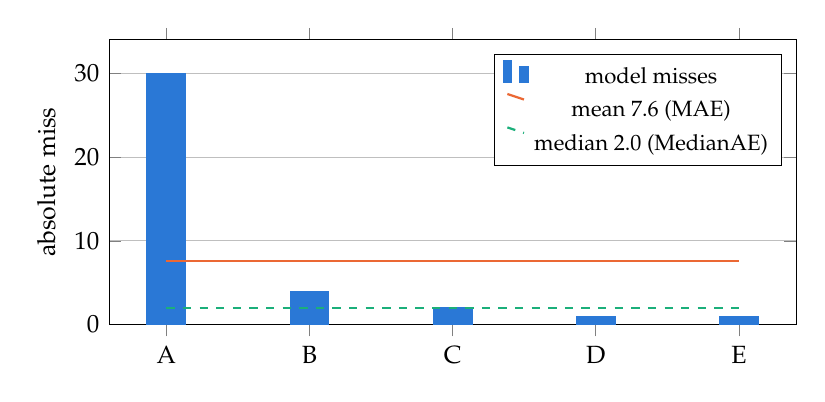
\begin{tikzpicture}
\begin{axis}[width=0.85\textwidth, height=5.2cm, ybar,
  symbolic x coords={A,B,C,D,E}, xtick=data,
  ylabel={absolute miss}, ymin=0, ymax=34,
  bar width=14pt, ymajorgrids, legend style={font=\footnotesize, at={(0.98,0.95)}, anchor=north east}]
\addplot[fill=kblue, draw=kblue] coordinates {(A,30) (B,4) (C,2) (D,1) (E,1)};
\addplot[korange, sharp plot, thick, no marks] coordinates {(A,7.6) (E,7.6)};
\addplot[kteal, sharp plot, thick, dashed, no marks] coordinates {(A,2) (E,2)};
\legend{model misses, mean 7.6 (MAE), median 2.0 (MedianAE)}
\end{axis}
\end{tikzpicture}
\caption{The five toy misses. One tall bar drags the mean to 7.6 while the
median stays at 2.0 with the typical country.}
\label{fig:metrics}
\end{figure}

\subsection{Two fairness rules}

The level and delta parameterizations (Equation 6): a model may be asked
either ``what will the level be'' or ``how much will it change,'' but if
it answers the second (say a predicted change of $+3$ from a level of
120), the level $120 + 3 = 123$ is reconstructed and scored. The
parameterization changes the question asked, never the quantity judged.
The same-rows rule: every model is scored on the identical set of rows,
because a model scored only on easy rows wins by taking a different exam.
Both rules are enforced in \texttt{evaluate.comparison\_table}.

\subsection{The trap}

The instinct is to ask which metric is best. The project's own test set
answers that this is the wrong question: \texttt{xgb\_delta} wins MAE
(9.345 against 11.004) while persistence wins MedianAE (1.367) on the same
predictions and the same rows. Neither verdict is an error. The right
question is which judge answers the question at hand: total misallocated
megatons is MAE's question; ``will this work for a typical country'' is
MedianAE's.

\subsection{Teach-back questions}

\begin{enumerate}
\item In the toy table, MAE is 7.6 and MedianAE is 2.0. Explain what each
number describes and why they differ by a factor of almost four.
\item A colleague reports ``our model achieved MAE 9.3, an excellent
result.'' What single number do you demand before accepting the claim?
\item Why is the $\tau = 1$ Mt exclusion part of MdAPE's definition rather
than optional cleaning? Use country E to show what would happen without it.
\item Using only MAE and RMSE from a comparison table, how would you
detect that a model is failing catastrophically on a few giants?
\end{enumerate}

\section{Lesson 2: The opponent. Baselines and knowing in advance where each fails}

\subsection{Concept}

A baseline is a forecast with zero fitted parameters: nothing in it is
estimated from data, so nothing in it can overfit or be tuned to flatter
itself. Its job is to define the bar. If a model with 17 features cannot
beat a rule a student can compute on paper, the machinery added nothing.

\subsection{Persistence (Equation 7)}

Persistence predicts that next year equals this year. Its miss is
therefore the data's own year-over-year change, which has two
consequences. First, persistence's MAE equals the average absolute annual
change of the series, so the bar every model must clear can be computed
before any model exists. Second, beating persistence means predicting the
direction and size of the change better than the guess ``zero change,''
which is a real demand, not a formality.

Persistence is the optimal forecast under a random walk, a series whose
next value is the current value plus an unpredictable step of mean zero
\cite{hyndman2021forecasting}. It is strong for CO$_2$ specifically
because emissions come from physical stock (power plants, vehicle fleets,
industrial capital) that cannot change quickly: in this dataset the
median absolute year-over-year change since 2010 is about 4.4 percent of
the level (Session 1 EDA).

\subsection{Linear trend, or drift (Equation 8)}

Drift measures the average yearly change over the last five years and
assumes one more year of exactly that. Two invented countries make the
trade-off visible.

\emph{A sustained riser:} emissions 80, 84, 88, 92, 96, 100 over six
years. The five-year slope is $(100-80)/5 = +4$ per year, so drift
predicts 104 and persistence predicts 100. If the actual value is 104,
drift's miss is 0 and persistence's is 4.

\emph{A country that peaked:} emissions 90, 94, 98, 102, then a turn:
100, 98. The five-year slope is $(98-90)/5 = +1.6$, still positive two
years after the peak, because the window still contains the boom years.
Drift predicts 99.6, persistence predicts 98, and the actual value falls
to 95. Persistence misses by 3; drift misses by 4.6 and points in the
wrong direction. A five-year window remembers old growth long after
reality has moved on.

\begin{figure}[ht]
\centering
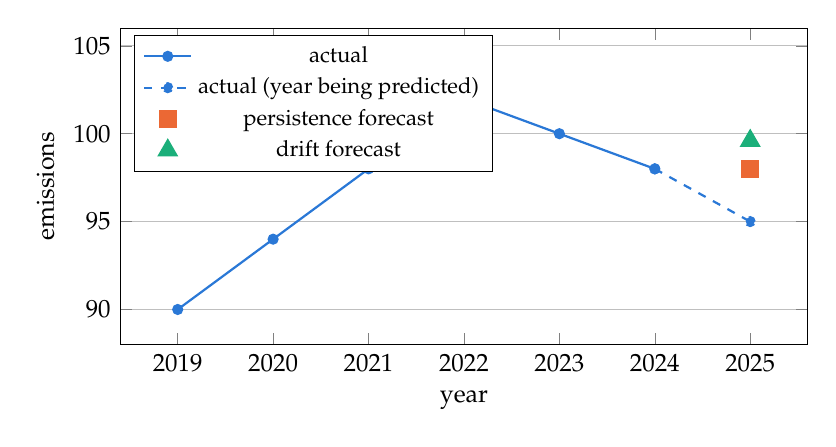
\begin{tikzpicture}
\begin{axis}[width=0.85\textwidth, height=5.6cm,
  xlabel={year}, ylabel={emissions},
  xtick={2019,2020,2021,2022,2023,2024,2025},
  x tick label style={/pgf/number format/1000 sep=},
  ymin=88, ymax=106, ymajorgrids,
  legend style={font=\footnotesize, at={(0.02,0.98)}, anchor=north west}]
\addplot[kblue, thick, mark=*, mark size=1.6pt] coordinates
  {(2019,90) (2020,94) (2021,98) (2022,102) (2023,100) (2024,98)};
\addplot[kblue, thick, dashed, mark=*, mark size=1.6pt] coordinates
  {(2024,98) (2025,95)};
\addplot[only marks, mark=square*, korange, mark size=3pt] coordinates {(2025,98)};
\addplot[only marks, mark=triangle*, kteal, mark size=4pt] coordinates {(2025,99.6)};
\legend{actual, actual (year being predicted), persistence forecast, drift forecast}
\end{axis}
\end{tikzpicture}
\caption{The peaked country. Drift's stale positive slope points upward
two years after the turn; persistence misses less.}
\label{fig:turn}
\end{figure}

\subsection{Bias direction, and the real echoes}

For a trending country, persistence's misses lean in a predictable
direction: it under-predicts a riser every year and over-predicts a
decliner every year, with the sign of the bias tracking the country's own
recent trend. This allows failure predictions before any computation:
persistence systematically under-shot Qatar, which rose every year from
2020 to 2024 (101.3 to 125.8 Mt), and over-shot sustained decliners such
as Germany.

On the real validation years, drift won in 39.2 percent of countries (the
steady decliners) and persistence won the rest; overall MAE was 6.757 for
persistence against 7.281 for drift, yet drift won MedianAE and MdAPE,
with persistence's advantage concentrated in avoiding disasters among
giants (RMSE 24.9 against 33.3). The COVID shock is the peaked-country
example at scale, with a timing twist: persistence's worst test year was
2020 itself, while drift's was 2021, because the 2020 collapse had by
then entered drift's slope window and poisoned it just as emissions
rebounded.

\subsection{The trap}

Students meet baselines and conclude they are a formality. The project's
actual result is the antidote: on validation no learned model beat
persistence at all (best skill $-0.017$), and on test the best model's
win was statistically indistinguishable from zero (Lesson 5). Any report
of model MAE without a persistence bar has hidden the hardest question:
what would doing nothing have scored?

\subsection{Teach-back questions}

\begin{enumerate}
\item Persistence's miss equals the country's actual year-over-year
change. Explain why, and state what beating persistence therefore demands.
\item For a country whose emissions peaked in 2010 and have declined
steadily since, which direction does persistence miss, and which baseline
should win there? What event would flip the winner back to persistence?
\item Using the peaked-country example, explain mechanically why drift's
worst real test year was 2021 rather than 2020.
\end{enumerate}

\section{Lesson 3: The first learner. Ordinary least squares and Ridge}

\subsection{The scoring machine, and what S(beta) means}

We predict this year's emissions from one feature, last year's emissions,
using three rows of invented data:

\begin{center}
\begin{tabular}{lrr}
\toprule
Row & Last year (feature) & This year (actual) \\
\midrule
1 & 10 & 10.5 \\
2 & 20 & 21 \\
3 & 40 & 42 \\
\bottomrule
\end{tabular}
\end{center}

The model is: prediction $= \beta \times$ last year, where $\beta$ is one
weight to be chosen. Persistence is the special case $\beta = 1$ imposed
by decree; a learned model lets the data choose $\beta$.

Define a scoring machine $S$: feed it one candidate weight, and it makes
all three predictions, measures the misses, squares them, and adds them
up. The notation $S(1)$ reads ``$S$ of 1,'' the machine's score for the
input 1; the parentheses are function notation, not multiplication.
Running the machine by hand:
\[
S(1) = 0.5^2 + 1^2 + 2^2 = 5.25, \qquad
S(0.95) = 1^2 + 2^2 + 4^2 = 21, \qquad
S(1.05) = 0 .
\]

\subsection{OLS (Equation 9): report the arg min}

Feeding the machine many weights produces a bowl-shaped curve
(Figure~\ref{fig:bowl}). Two different questions can be asked of the
bowl. The \emph{min} asks how low the curve goes (here 0, a height); the
\emph{arg min} asks at which weight it goes that low (here 1.05, a
position). Equation 9 of the foundations document instructs: report the
arg min. The output of least squares is a weight, not an error value.

\begin{figure}[ht]
\centering
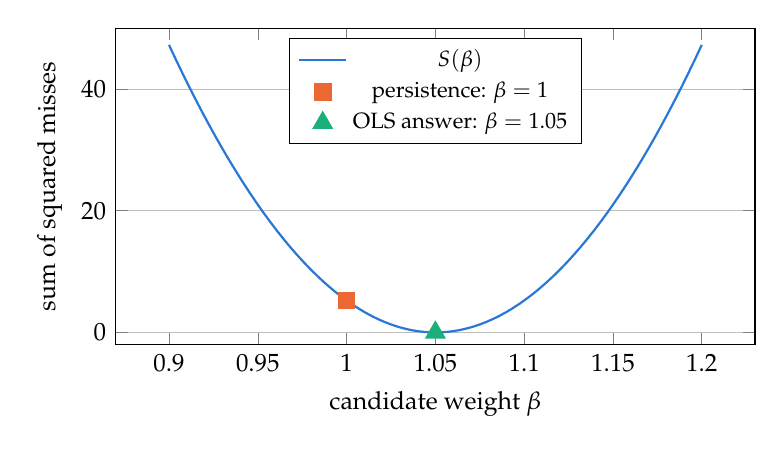
\begin{tikzpicture}
\begin{axis}[width=0.8\textwidth, height=5.6cm,
  xlabel={candidate weight $\beta$}, ylabel={sum of squared misses},
  ymin=-2, ymax=50, ymajorgrids,
  legend style={font=\footnotesize, at={(0.5,0.97)}, anchor=north}]
\addplot[kblue, thick, domain=0.9:1.2, samples=80] {2100*(1.05-x)^2};
\addplot[only marks, mark=square*, korange, mark size=3pt] coordinates {(1.0,5.25)};
\addplot[only marks, mark=triangle*, kteal, mark size=4pt] coordinates {(1.05,0)};
\legend{$S(\beta)$, persistence: $\beta=1$, OLS answer: $\beta=1.05$}
\end{axis}
\end{tikzpicture}
\caption{The bowl. The min is the height 0; the arg min is the position
1.05; least squares reports the position.}
\label{fig:bowl}
\end{figure}

The closed form (Equation 11) is a division in disguise: the sum of
feature times answer ($10 \times 10.5 + 20 \times 21 + 40 \times 42 =
2205$) divided by the sum of feature times feature ($100 + 400 + 1600 =
2100$), giving $\hat\beta = 2205/2100 = 1.05$. Read it as co-movement
divided by self-movement. With 17 features the division becomes a matrix
inverse, but the meaning is unchanged. In real data the bowl's bottom
never touches zero; the toy rows were invented to fit perfectly.

\subsection{Ridge (Equations 10 and 11): a price on weight size}

The project's feature set contains near-twin columns
(\texttt{co2\_lag1}, \texttt{co2\_roll5\_mean}). When two columns carry
almost the same information, OLS cannot decide how to split the weight
between them: $+30$ on one twin and $-29$ on the other fits the training
data about as well as $0.5$ and $0.5$, so the fitted weights swing wildly
with tiny changes in the data. Ridge changes one thing: the scoring
machine now charges for two items,
\[
\text{ridge score} = \text{(sum of squared misses)} +
\alpha \times \text{(sum of squared weights)} ,
\]
where $\alpha \ge 0$ is the price level. Among weight combinations that
fit equally well, Ridge picks the smallest ($0.5^2 + 0.5^2 = 0.5$ is far
cheaper than $30^2 + 29^2 = 1741$), so near-twins share their weight
instead of fighting over it. The addition of $\alpha$ inside the closed
form also guarantees that the division always works
\cite{hoerl1970ridge}. In the one-feature example the best weight becomes
$2205 / (2100 + \alpha)$: raising $\alpha$ shrinks the weight toward
zero, and at extreme $\alpha$ the model degenerates into predicting the
same constant for everyone.

\begin{figure}[ht]
\centering
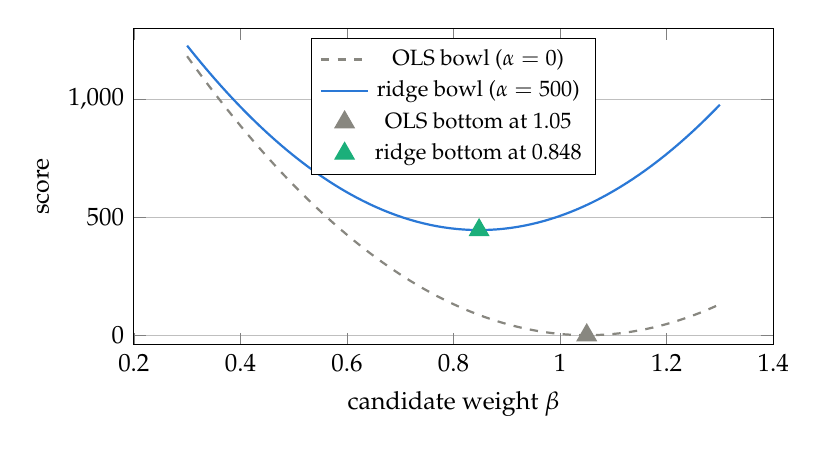
\begin{tikzpicture}
\begin{axis}[width=0.8\textwidth, height=5.6cm,
  xlabel={candidate weight $\beta$}, ylabel={score},
  ymin=-40, ymax=1300, ymajorgrids,
  legend style={font=\footnotesize, at={(0.5,0.97)}, anchor=north}]
\addplot[kgray, thick, dashed, domain=0.3:1.3, samples=80] {2100*(1.05-x)^2};
\addplot[kblue, thick, domain=0.3:1.3, samples=80] {2100*(1.05-x)^2 + 500*x^2};
\addplot[only marks, mark=triangle*, kgray, mark size=4pt] coordinates {(1.05,0)};
\addplot[only marks, mark=triangle*, kteal, mark size=4pt] coordinates {(0.848,445.2)};
\legend{OLS bowl ($\alpha=0$), ridge bowl ($\alpha=500$), OLS bottom at $1.05$, ridge bottom at $0.848$}
\end{axis}
\end{tikzpicture}
\caption{Adding the penalty bowl moves the combined bottom toward zero:
the arg min slides from 1.05 to $2205/2600 = 0.848$ at $\alpha = 500$.}
\label{fig:ridgebowl}
\end{figure}

Two footnotes complete the section. The penalty charges every weight the
same price per unit of size, so features must be standardized to
comparable scales first, with the scaler fit on training rows only.
And $\alpha$ is chosen by validation, not theory: Session 4 tried 0.1, 1,
10, 100 and validation MAE worsened as $\alpha$ grew (7.29, 7.53, 8.58,
9.95 for the level model), so the project froze $\alpha = 0.1$: a whisper
of penalty, enough to steady the twins without distorting the signal.

\subsection{Teach-back questions}

\begin{enumerate}
\item Inside $S(\beta)$, what is being squared and summed, row by row?
\item In the bowl picture, which number is the min, which is the arg min,
and which one is the fitted weight?
\item Persistence uses $\beta = 1$ and OLS found $\beta = 1.05$. What did
OLS learn that persistence assumes away?
\item A colleague sets $\alpha$ to one million. What happens to the
weights, and what forecast does the model degenerate into?
\end{enumerate}

\section{Lesson 4: The heavy machinery. Trees, bagging, boosting, XGBoost}

\subsection{Trees (Equation 12): staircases with a ceiling}

A tree asks yes-or-no questions (``is last year's emissions 50 or
more?'') and predicts, within each resulting group, the group's average.
Choosing the average is not arbitrary: it is the value minimizing the sum
of squared misses within the group, the same bowl as always, applied per
group. Two consequences follow. Trees need no feature scaling, because a
threshold question cares only about the ordering of values, not their
units. And a tree cannot predict outside what it has seen: every
prediction is an average of training answers, so the prediction surface
is a staircase, and the staircase has a top step
(Figure~\ref{fig:staircase}).

\begin{figure}[ht]
\centering
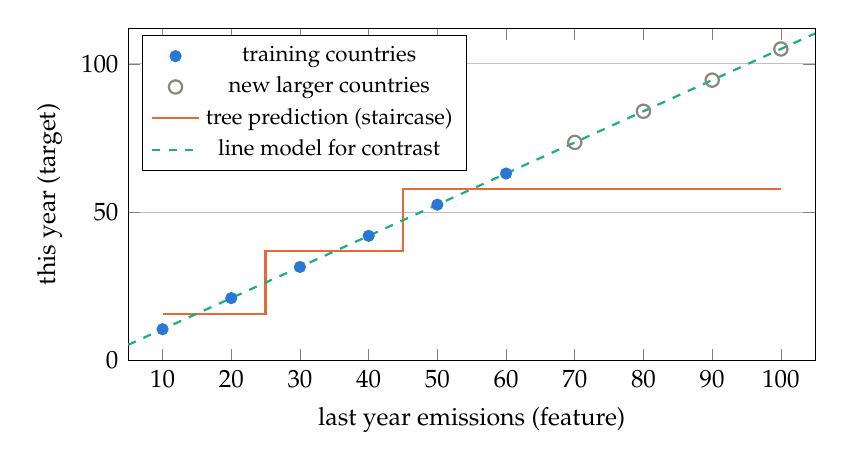
\begin{tikzpicture}
\begin{axis}[width=0.85\textwidth, height=5.8cm,
  xlabel={last year emissions (feature)}, ylabel={this year (target)},
  ymin=0, ymax=112, xmin=5, xmax=105, ymajorgrids,
  legend style={font=\footnotesize, at={(0.02,0.98)}, anchor=north west}]
\addplot[only marks, mark=*, kblue, mark size=2pt] coordinates
  {(10,10.5) (20,21) (30,31.5) (40,42) (50,52.5) (60,63)};
\addplot[only marks, mark=o, kgray, mark size=2.4pt, thick] coordinates
  {(70,73.5) (80,84) (90,94.5) (100,105)};
\addplot[korange, thick, const plot, no marks] coordinates
  {(10,15.75) (25,36.75) (45,57.75) (100,57.75)};
\addplot[kteal, thick, dashed, domain=5:105, samples=2] {1.05*x};
\legend{training countries, new larger countries, tree prediction (staircase), line model for contrast}
\end{axis}
\end{tikzpicture}
\caption{Inside the training range the staircase tracks the data; beyond
it, the tree stays flat at its top step while the truth keeps rising.}
\label{fig:staircase}
\end{figure}

\subsection{Bagging (Equation 13) and boosting (Equations 14 and 15)}

Bagging fits many trees, each on a bootstrap resample of the training
rows, and averages their predictions: a parallel committee whose
individual quirks cancel \cite{breiman1996bagging}. Random forests
additionally restrict each split to a random subset of features so the
committee members disagree more \cite{breiman2001random}.

Boosting is instead a sequential relay: the model is a sum of many small
trees built one at a time, and each new tree is trained on the leftovers
(the residuals, actual minus current prediction) of the team so far
\cite{friedman2001greedy}. With one country whose actual value is 100:
tree 1 predicts 90 (leftover 10), tree 2 adds 7 (total 97), tree 3 adds 2
(total 99), tree 4 adds 0.7. Each tree is weak; the sum creeps toward the
target (Figure~\ref{fig:relay}). Scikit-learn's
\texttt{HistGradientBoostingRegressor} is this machine with feature
values binned into histograms.

\begin{figure}[ht]
\centering
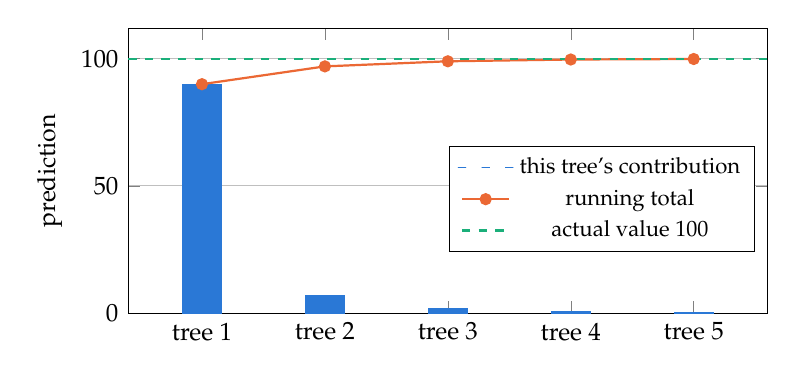
\begin{tikzpicture}
\begin{axis}[width=0.8\textwidth, height=5.2cm,
  xlabel={}, ylabel={prediction},
  xtick={1,2,3,4,5},
  xticklabels={tree 1, tree 2, tree 3, tree 4, tree 5},
  ymin=0, ymax=112, xmin=0.4, xmax=5.6, ymajorgrids,
  legend style={font=\footnotesize, at={(0.98,0.4)}, anchor=east}]
\addplot[ybar, bar width=14pt, fill=kblue, draw=kblue] coordinates
  {(1,90) (2,7) (3,2) (4,0.7) (5,0.2)};
\addplot[korange, thick, mark=*, mark size=1.8pt] coordinates
  {(1,90) (2,97) (3,99) (4,99.7) (5,99.9)};
\addplot[kteal, thick, dashed, no marks] coordinates {(0.4,100) (5.6,100)};
\legend{this tree's contribution, running total, actual value 100}
\end{axis}
\end{tikzpicture}
\caption{The boosting relay: shrinking corrections, a running total that
creeps toward the target.}
\label{fig:relay}
\end{figure}

\subsection{XGBoost (Equations 16 to 24): rooms, leftovers, and prices}

XGBoost is the relay plus the idea from Ridge: complexity must be paid
for \cite{chen2016xgboost}. The vocabulary, grounded in one concrete
walkthrough. Freeze the relay mid-work, with four countries:

\begin{center}
\begin{tabular}{lrrr}
\toprule
Country & Actual & Team predicts so far & Leftover \\
\midrule
A & 100 & 90 & $+10$ \\
B & 60  & 46 & $+14$ \\
C & 20  & 22 & $-2$ \\
D & 12  & 16 & $-4$ \\
\bottomrule
\end{tabular}
\end{center}

The new tree asks one question (``is last year's emissions 50 or
more?''), which sorts A and B into one group and C and D into another. A
\emph{room} (the formal term is a leaf) is such a group, and each room
hands one shared correction to its members. Plain boosting uses the
room's average leftover: $+12$ for the first room, $-3$ for the second.
XGBoost multiplies the average by $n/(n+\lambda)$, where $n$ is the
number of rows in the room: with $\lambda = 1$, the corrections become
$12 \times 2/3 = +8$ and $-3 \times 2/3 = -2$ (Equation 22). This
\emph{evidence shrink} is Ridge's philosophy relocated into every room:
a room holding two odd country-years is heavily damped, while a room
holding 100 rows keeps almost its full correction
(Figure~\ref{fig:shrink}). The dictionary:

\begin{center}
\begin{tabular}{lll}
\toprule
Plain word & In the walkthrough & Formal term \\
\midrule
Leftover & the column actual $-$ predicted & residual \\
Room & the group $\{A, B\}$ or $\{C, D\}$ & leaf \\
Correction & the room's one number, $+8$ or $-2$ & leaf weight $w$ \\
Shrink & the multiplier $2/(2+1)$ & $n/(n+\lambda)$, Eq.~22 \\
Rent & the entry fee a new split must pay & $\gamma$, Eqs.~16, 21 \\
Pace & scale each correction by 0.10 & learning rate $\eta$, Eq.~23 \\
\bottomrule
\end{tabular}
\end{center}

\begin{figure}[ht]
\centering
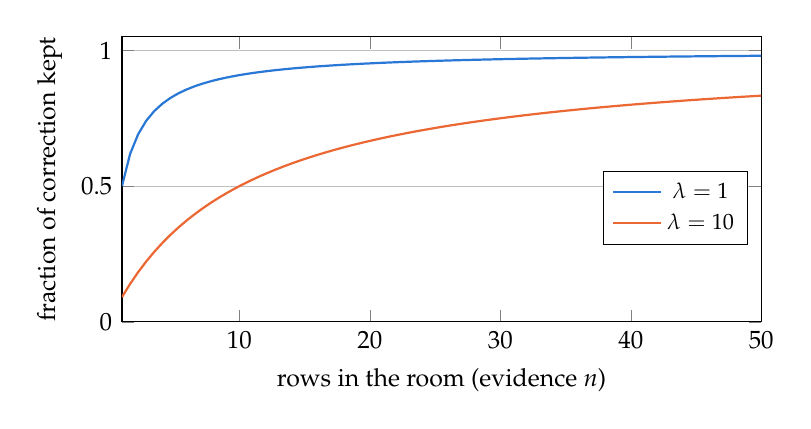
\begin{tikzpicture}
\begin{axis}[width=0.8\textwidth, height=5.2cm,
  xlabel={rows in the room (evidence $n$)}, ylabel={fraction of correction kept},
  ymin=0, ymax=1.05, xmin=1, xmax=50, ymajorgrids,
  legend style={font=\footnotesize, at={(0.98,0.4)}, anchor=east}]
\addplot[kblue, thick, domain=1:50, samples=80] {x/(x+1)};
\addplot[korange, thick, domain=1:50, samples=80] {x/(x+10)};
\legend{$\lambda = 1$, $\lambda = 10$}
\end{axis}
\end{tikzpicture}
\caption{The evidence shrink $n/(n+\lambda)$. Thin-evidence rooms are
damped hardest; well-evidenced rooms pass almost untouched.}
\label{fig:shrink}
\end{figure}

Three more pieces complete the machine. The \emph{rent} $\gamma$: a
candidate split is scored by the improvement it brings minus $\gamma$
(Equation 21), so a split improving the objective by 7 with rent 4 is
made (net $+3$) while one improving by 2 is never born (net $-2$); this
prunes memorization such as single-country rooms. The \emph{learning
rate} $\eta$: each finished tree enters the team scaled by $\eta$
(Equation 23), so with the project's $\eta = 0.10$ the first room's $+8$
enters as $+0.8$ and the relay compensates by running many trees.
\emph{Early stopping} (Equation 24): trees are added while the validation
MAE improves and the count is frozen at the best point $M^*$
(Figure~\ref{fig:earlystop}); the model is then refit on training plus
validation rows with the count locked and early stopping disabled, so the
test years never influence any choice. The project's frozen
configuration: \texttt{xgb\_delta}, depth 3, $\eta = 0.10$, $M^* = 173$
trees. A software footnote: the xgboost implementation reports split
gains without the constant one half of Equation 21, which never changes
which split wins; the foundations document verified this against xgboost
3.3.0 on a worked example.

\begin{figure}[ht]
\centering
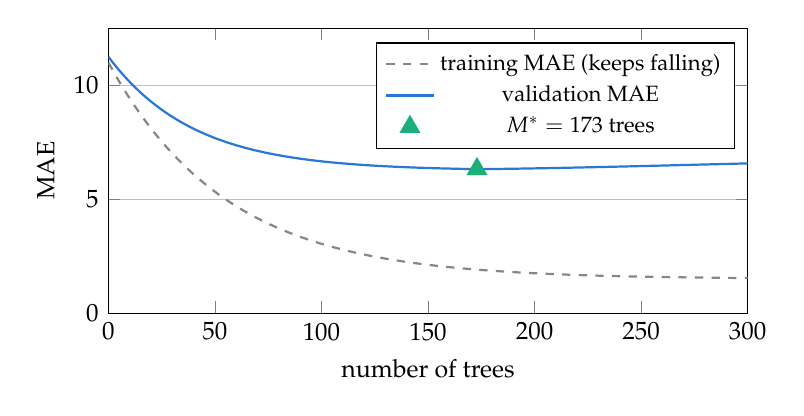
\begin{tikzpicture}
\begin{axis}[width=0.8\textwidth, height=5.2cm,
  xlabel={number of trees}, ylabel={MAE},
  ymin=0, ymax=12.5, xmin=0, xmax=300, ymajorgrids,
  legend style={font=\footnotesize, at={(0.98,0.95)}, anchor=north east}]
\addplot[kgray, thick, dashed, domain=0:300, samples=100] {1.5 + 9.5*exp(-x/55)};
\addplot[kblue, thick, domain=0:300, samples=120] {6.25 + 5*exp(-x/40) + 0.0025*max(0,x-173)};
\addplot[only marks, mark=triangle*, kteal, mark size=4pt] coordinates {(173,6.32)};
\legend{training MAE (keeps falling), validation MAE, $M^* = 173$ trees}
\end{axis}
\end{tikzpicture}
\caption{Early stopping, illustrative curve shapes. Training error falls
forever; validation error bottoms out where memorization begins. The
project's real frozen count is 173.}
\label{fig:earlystop}
\end{figure}

\subsection{Why trees require the delta parameterization}

The staircase ceiling meets the test set: countries whose emissions rose
above anything in training saturate a level-parameterized tree, which
then systematically under-predicts every growing giant. This is visible
in the real results: \texttt{hgb\_level} posted validation RMSE 142.7,
and \texttt{xgb\_level} was the one model that significantly lost to
persistence on test (skill $-1.834$, $p = 0.005$). The delta
parameterization sidesteps the ceiling: the tree predicts the bounded
year-over-year change, well within training experience, and the level is
reconstructed from the known current value. The unbounded part comes from
the data; the tree handles only the bounded part.

\subsection{Teach-back questions}

\begin{enumerate}
\item A room contains three countries with leftovers $+6$, $+9$, and
$+9$, and $\lambda = 1$. What correction does plain boosting hand out,
and what correction does XGBoost hand out?
\item Ridge's $\alpha$ and XGBoost's $\lambda$ are the same idea deployed
in different places. What does each one shrink?
\item A student asks why not always use the line model, since it
extrapolates. Give one honest sentence for each side.
\item Why does the project's protocol allow validation to choose the tree
count but never the test years?
\end{enumerate}

\section{Lesson 5: Is the win real? Uncertainty of a skill score}

\subsection{Concept}

The test result says \texttt{xgb\_delta} has skill $+0.151$. But that
number was computed on one particular sample: the 153 countries that
exist, over five particular test years. Six heads in ten coin flips does
not prove a biased coin; the question is how much the skill would wobble
if the world had dealt a slightly different set of countries.

\subsection{The loss differential (Equation 25), and why rows are not independent}

For every row, subtract the model's miss from persistence's miss; a
positive difference means the model won that row
\cite{diebold1995comparing}. Four example rows expose the key problem:

\begin{center}
\begin{tabular}{lrrr}
\toprule
Row & Persistence miss & Model miss & Difference $d$ \\
\midrule
China 2019 & 20 & 12 & $+8$ \\
China 2020 & 30 & 24 & $+6$ \\
Qatar 2019 & 4 & 5 & $-1$ \\
Qatar 2020 & 3 & 5 & $-2$ \\
\bottomrule
\end{tabular}
\end{center}

China's rows are both positive; Qatar's are both negative. Rows travel in
country packs: a model that understands China's dynamics wins all five of
China's test years together. So China's five rows are one witness
interviewed five times, not five independent witnesses. The test set has
762 rows but only 153 countries, and the honest amount of evidence is
closer to 153. Treating rows as independent would overstate the
certainty, which is why a row-level interval is wrong for this panel.

\subsection{The country-clustered bootstrap (Equations 26 to 28)}

The fix is a resampling game played at the country level
\cite{efron1993bootstrap, cameron2008bootstrap}. One round: put the 153
country names in a hat; draw 153 names with replacement (some countries
repeat, some sit out); pool every test row of the drawn countries and
recompute the skill (Equation 26). Repeat 2000 times. Because whole
countries are drawn, each country's years stay together and the
family-pack correlation is preserved. The spread of the 2000 replicate
skills is the wobble. The 95 percent confidence interval is the range
from the 2.5th to the 97.5th percentile of the replicates (Equation 27),
and the p-value is twice the fraction of replicates on the wrong side of
zero (Equation 28).

\begin{figure}[ht]
\centering
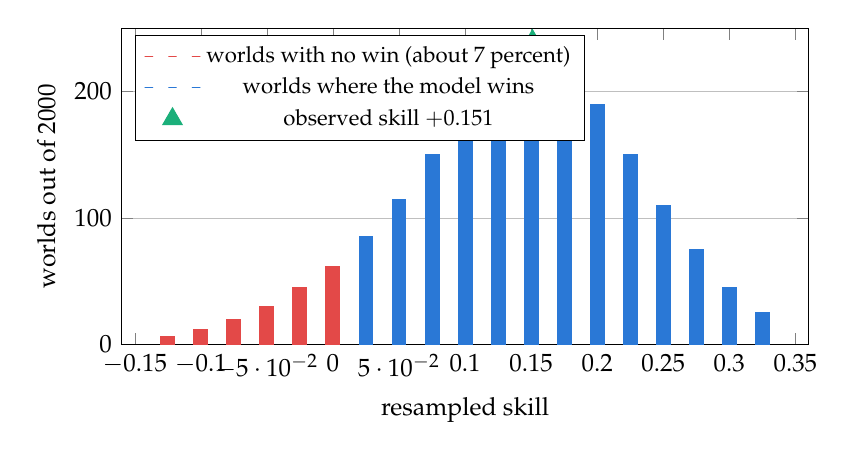
\begin{tikzpicture}
\begin{axis}[width=0.85\textwidth, height=5.6cm,
  xlabel={resampled skill}, ylabel={worlds out of 2000},
  ymin=0, ymax=250, xmin=-0.16, xmax=0.36, ymajorgrids,
  legend style={font=\footnotesize, at={(0.02,0.98)}, anchor=north west}]
\addplot[ybar, bar width=5pt, fill=kred, draw=kred] coordinates
  {(-0.125,6) (-0.10,12) (-0.075,20) (-0.05,30) (-0.025,45) (0.0,62)};
\addplot[ybar, bar width=5pt, fill=kblue, draw=kblue] coordinates
  {(0.025,85) (0.05,115) (0.075,150) (0.10,185) (0.125,210) (0.15,225)
   (0.175,215) (0.20,190) (0.225,150) (0.25,110) (0.275,75) (0.30,45) (0.325,25)};
\addplot[only marks, mark=triangle*, kteal, mark size=4pt] coordinates {(0.151,240)};
\legend{worlds with no win (about 7 percent), worlds where the model wins, observed skill $+0.151$}
\end{axis}
\end{tikzpicture}
\caption{Illustrative sketch of the bootstrap distribution for the real
headline result. The interval and p-value are the project's real numbers;
the histogram shape is a sketch consistent with them.}
\label{fig:hist}
\end{figure}

\subsection{The verdicts in honest English}

Three from the real project. First, \texttt{xgb\_delta} on test: skill
$+0.151$, interval $[-0.018, +0.271]$, $p = 0.14$; the honest sentence is
that the point estimate favors the model but the evidence cannot rule
out a tie with persistence. Second, linear trend on validation: skill
$-0.078$, interval $[-0.34, +0.20]$, $p \approx 0.7$; not ``trend
loses'' but ``trend and persistence are statistically indistinguishable
on this sample.'' Third, \texttt{xgb\_level} on test: skill $-1.834$,
$p = 0.005$, the one settled verdict in the table, and it is a loss. The
symmetry worth teaching: the skill score keeps a model honest against
doing nothing, and the bootstrap keeps the skill score honest against
luck.

\subsection{Teach-back questions}

\begin{enumerate}
\item A journalist writes ``the model beat the baseline by 15 percent.''
Using the first verdict above, write the one-sentence correction.
\item Why are countries, not rows, resampled? What would a row-level
resample destroy?
\item What does it mean that the interval $[-0.018, +0.271]$ contains
zero?
\end{enumerate}

\section{Lesson 6: Where does the win live? Error decomposition}

\subsection{Group MAE and within-group skill (Equations 29 and 30)}

No new machinery: slice the test rows into groups (years, countries, or
emitter-size tiers), compute the ordinary MAE inside each group, and
judge each group against persistence's error in that same group. Each
tier gets its own honest contest with the bar set locally.

\subsection{The trap this section exists to expose}

Six invented countries in two tiers:

\begin{center}
\begin{tabular}{lrll}
\toprule
Tier & Rows & Persistence misses & Model misses \\
\midrule
Giant & 2 & 100, 100 & 60, 60 \\
Small & 4 & 2, 2, 2, 2 & 4, 4, 4, 4 \\
\bottomrule
\end{tabular}
\end{center}

Giant tier: model MAE 60 against 100, skill $+0.40$. Small tier: model
MAE 4 against 2, skill $-1.0$; the model is twice as bad. Overall:
persistence total error 208, model total 136, overall skill
$1 - 136/208 = +0.35$. The model is worse for four of the six countries,
the clear majority, yet the overall number looks excellent, because the
error mass lives in the two giants. A single headline cannot distinguish
``wins everywhere'' from ``wins where the tonnage is.''

The real project mirrors the toy almost exactly
(Figure~\ref{fig:tiers}): the headline test skill of $+0.151$ decomposes
into giant tier (25 rows at 1000 Mt and above) skill $+0.325$, large and
mid tiers approximately zero, and small tier $-0.863$, where every
learned model loses to persistence. The deployment claim must be
tier-scoped. By year, the same equation shows \texttt{xgb\_delta} with
positive skill in all five test years but earning most in calm 2019 and
2022, so the gain reads as steady-state structure rather than shock
anticipation.

\begin{figure}[ht]
\centering
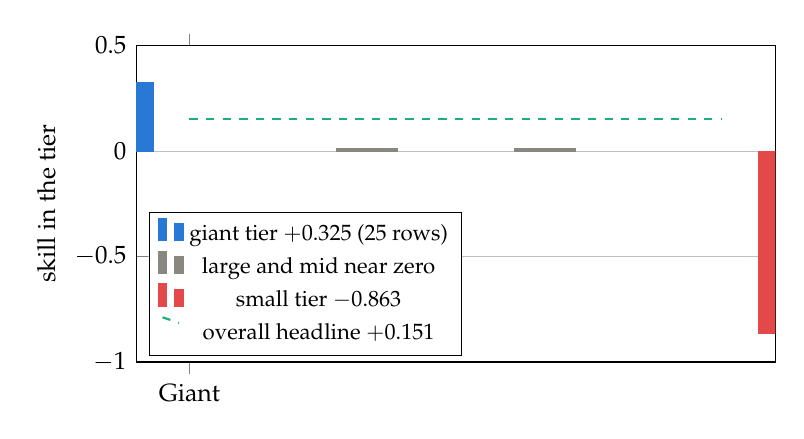
\begin{tikzpicture}
\begin{axis}[width=0.8\textwidth, height=5.6cm, ybar,
  symbolic x coords={Giant, Large, Mid, Small}, xtick=data,
  ylabel={skill in the tier}, ymin=-1.0, ymax=0.5, ymajorgrids,
  bar width=22pt,
  legend style={font=\footnotesize, at={(0.02,0.02)}, anchor=south west}]
\addplot[fill=kblue, draw=kblue] coordinates {(Giant,0.325)};
\addplot[fill=kgray, draw=kgray] coordinates {(Large,0.01) (Mid,0.01)};
\addplot[fill=kred, draw=kred] coordinates {(Small,-0.863)};
\addplot[kteal, sharp plot, thick, dashed, no marks] coordinates {(Giant,0.151) (Small,0.151)};
\legend{giant tier $+0.325$ (25 rows), large and mid near zero, small tier $-0.863$, overall headline $+0.151$}
\end{axis}
\end{tikzpicture}
\caption{The real test-set decomposition. The overall headline sits
between the tiers and describes none of them.}
\label{fig:tiers}
\end{figure}

\subsection{Permutation importance (Equation 31), and the twin caveat}

To ask whether the model relied on feature $j$, shuffle column $j$ across
the evaluation rows, destroying its information while preserving its
distribution, and measure how much the error rises
\cite{breiman2001random}. The caveat follows from Lesson 3's twins: when
two features carry overlapping information, shuffling one lets the model
lean on the other, so both can score near zero even when their shared
signal is essential. The real numbers show it: the five-year slope ranks
first (2.889, unique directional information), while
\texttt{co2\_roll5\_mean} scores just 0.098, not because the level family
is useless but because it is redundant. Importances over correlated
features describe group structure, never a per-feature verdict, and no
feature is added or dropped in response, since the configuration is
frozen post-test.

\subsection{Teach-back questions}

\begin{enumerate}
\item A ministry official from a small emitting country asks whether to
adopt the model for national projections. Give the two-sentence honest
answer using the tier figure.
\item Construct in words a situation where overall skill is positive
while the model loses in most groups. What makes it possible?
\item Two features both score near zero permutation importance. Give two
different explanations, and say what additional check separates them.
\end{enumerate}

\section{The whole document in six sentences}

First, a miss can be counted five ways, and the choice of judge is itself
a modeling decision; no metric is neutral. Second, persistence's error is
the data's own year-over-year change, so the bar to clear is computable
before any model exists, and for slow-moving CO$_2$ that bar is high.
Third, OLS walks to the bottom of the squared-miss bowl, and Ridge adds a
price on weight size, trading a small bias for stability when features
are near-twins. Fourth, trees are staircases with a ceiling, boosting is
a relay of corrections, and XGBoost is that relay with rent on rooms, an
evidence shrink on every correction, and a validation-chosen stopping
point; the ceiling is why the delta parameterization wins. Fifth, rows
travel in country packs, so whole countries are resampled, and the honest
headline is a point estimate whose interval includes zero. Sixth, the win
lives almost entirely in 25 giant rows while small emitters are better
served by no model at all, and importances over twins describe groups,
not features.

\appendix

\section{Model answers to the teach-back questions}

\textbf{Lesson 1.} (1) MAE is the tonnage-weighted average miss and is
dominated by country A; MedianAE is the middle miss and reports the
typical country; they differ because the errors are concentrated. (2) The
persistence MAE on the same rows: without the bar, 9.3 is uninterpretable.
(3) Percentage error divides by the level, which explodes as the level
approaches zero; without the threshold, country E alone would drag the
metric toward 200 percent. (4) An RMSE far above MAE signals that the
error budget is concentrated in a few large misses.

\textbf{Lesson 2.} (1) Persistence predicts last year's value, so its
miss is exactly the change; beating it means forecasting the change
better than guessing zero change. (2) Persistence over-predicts a
decliner; drift should win; a sudden reversal (a rebound, a shock) flips
the winner back to persistence. (3) In 2021 the 2020 collapse sat inside
drift's five-year window, dragging its slope downward just as emissions
rebounded; the window is a memory that a shock poisons for years.

\textbf{Lesson 3.} (1) The per-row misses, actual minus predicted. (2)
The min is 0, the arg min is 1.05, and the fitted weight is the arg min.
(3) That these countries grow about five percent per year. (4) All
weights are pushed essentially to zero and the model degenerates into
predicting the same constant for every country.

\textbf{Lesson 4.} (1) Plain boosting: the average, $+8$. XGBoost:
$8 \times 3/4 = +6$. (2) $\alpha$ shrinks the regression's feature
weights globally; $\lambda$ shrinks each room's correction, in proportion
to how little evidence the room contains. (3) The staircase captures
interactions and thresholds no single line can, but it cannot predict
outside the training range; the line extrapolates, but only along one
straight direction. (4) Validation exists to make modeling choices; the
test set exists to be touched once, so any choice influenced by it would
turn the test into a second validation set.

\textbf{Lesson 5.} (1) ``The model's error was 15 percent lower as a
point estimate, but the 95 percent country-clustered interval includes
zero, so a tie with the no-change baseline cannot be ruled out.'' (2) A
country's years are correlated; row-level resampling would scatter them
and understate the variance. (3) That among plausible worlds implied by
the data, some show the model not winning; the gap is within sampling
noise.

\textbf{Lesson 6.} (1) ``For small emitters this model is worse than
assuming no change, with tier skill $-0.863$; the gains are concentrated
in the largest emitters, so I would not recommend it for your case.''
(2) A few groups with very large errors dominate the total while the
model loses slightly in many small-error groups; concentration of error
mass makes it possible. (3) Either the feature is useless, or it is a
twin of another feature that covers for it when shuffled; shuffling the
whole correlated group together separates the two cases.

\bibliographystyle{plain}
\bibliography{references}

\end{document}
